\chapter{Cruscotto di controllo della qualità} \label{sec:cruscotto}

\section{Varianza dell'impegno orario}
\begin{figure}[H]
    \centering
    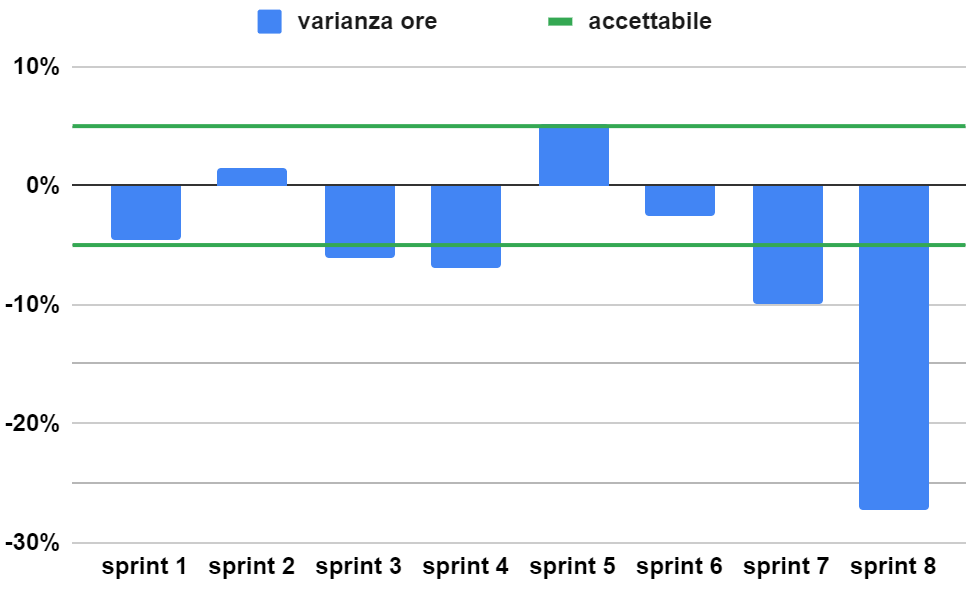
\includegraphics[width=0.8\linewidth]{VarOre.png}
    \caption{Varianza dell'impegno orario per sprint}
\end{figure}
\subsection{Analisi}
Analizzando i valori riportati nel grafico, è riscontrabile una difficoltà persistente nel produrre preventivi orari vicini al consuntivato.\\
In particolare, durante il periodo RTB, vengono registrati dei valori di poco inferiori all'accettabile nel terzo e quarto sprint e un valore di poco superiore nel quinto sprint. Il motivo del numero inferiore di ore produttive è stato causato da modifiche a documenti non previsti.\\
Valori di molto insufficienti sono stati registrati nel settimo e ottavo sprint. In questi casi, l'incompleta attività di progettazione è andata inevitabilmente ad impattare sulle task relative alla programmazione, rinviandone l'inizio dei lavori ai periodi successivi.

\section{Varianza di Budget}
\begin{figure}[H]
    \centering
    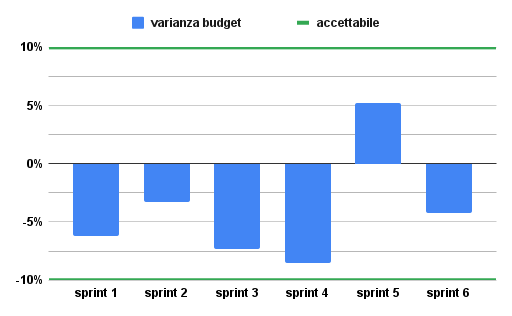
\includegraphics[width=0.8\linewidth]{VarBud.png}
    \caption{Varianza di Budget per sprint}
\end{figure}
\subsection{Analisi}
Dall'analisi del grafico è immediato osservare che i valori di varianza di budget sono sempre rimasti all'interno della soglia di accettabilità durante tutto il periodo RTB.\\
Il primo dato negativo e inferiore alla sogli di accettabilità è stato registrato durante l'ottavo sprint. In quel caso, come già analizzato con la Varianza dell'impegno orario, il mancato inizio delle attività di programmazione ha impattato sui costi, facendo sì che fosse di molto inferiore al preventivato.

\section{Estimate to Complete e Estimate at Completion}
\begin{figure}[H]
    \centering
    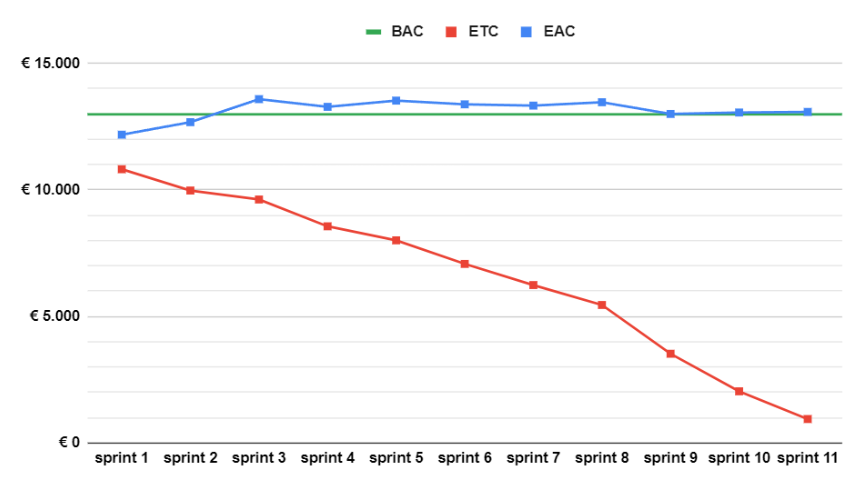
\includegraphics[width=0.8\linewidth]{ETCEAC.png}
    \caption{Progressione Estimate to Complete e Estimate at Completion in relazione al Budget at Completion}
\end{figure}
\subsection{Analisi}
Dopo un ottimo inizio nei primi due sprint, è possibile notare un calo dei lavori nel terzo sprint, e un altro leggero rallentamento nel quinto. L'Estimate to Complete al terzo e al quinto sprint è diminuito in modo meno marcato rispetto lo sprint precedente. Inoltre, l'Estimate at Completion ha superato il Budget at Completion.\\
Questo è causato dal mancato raggiungimento di tutti gli obiettivi fissati dalla milestone del terzo sprint.\\
Il valore dopo il terzo sprint, nonostante il brusco rallentamento dell'ottavo periodo di osservazione, è comunque rimasto stabile ad un valore poco al di sopra del Budget at Completion.

\section{Planned Value, Earned Value e Actual Cost}
\begin{figure}[H]
    \centering
    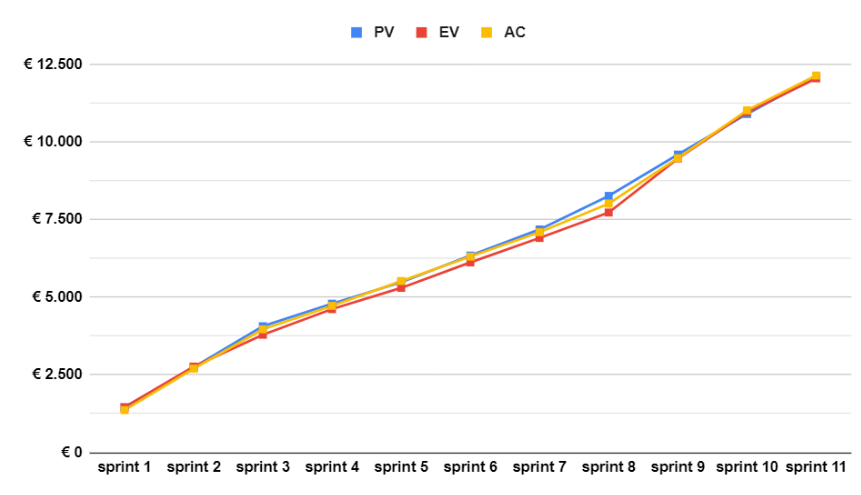
\includegraphics[width=0.8\linewidth]{PVEVAC.png}
    \caption{Progressione Planned Value, Earned Value e Actual Cost}
\end{figure}
\subsection{Analisi}
Dopo un ottimo inizio nei primi due sprint, come in altre metriche è possibile notare un calo dei lavori nel terzo. Se fino al secondo sprint i valori di Planned Value, Earned Value e Actual Cost erano quasi identici, a terzo sprint completato è riscontrabile dal cruscotto il "distaccamento" dei tre valori.\\
Questo è causato dal mancato raggiungimento di tutti gli obiettivi fissati dalla milestone del terzo sprint, che hanno portato l'Earned Value ad essere minore del Planned.\\
Dopo un andamento generalmente positivo tra il quarto e il settimo sprint ad avvicinare i valori delle tre metriche, Planned Value, Earned Value e Actual Cost hanno subito un ulteriore distaccamento durante l'ottavo periodo di osservazione. Questo è stato causato dall'elevata Varianza di budget e di impegno orario, già precedentemente analizzata.

\section{Schedule Variance e Cost Variance}
\begin{figure}[H]
    \centering
    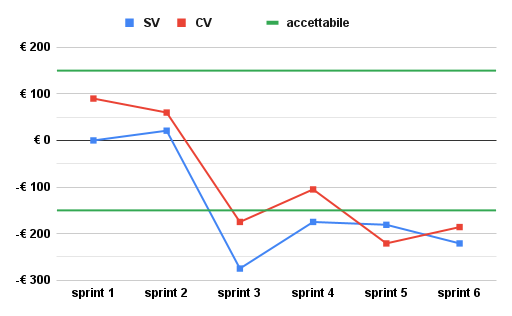
\includegraphics[width=0.8\linewidth]{SVCV.png}
    \caption{Progressione Schedule Variance e Cost Variance}
\end{figure}
\subsection{Analisi}
Dopo un ottimo inizio nei primi due sprint, come in altre metriche è possibile notare un calo dei lavori nel terzo. Se fino al secondo sprint i valori di Schedule e Cost Variance mostravano un anticipo sui lavori rispetto il costo preventivato per eseguirli, il mancato raggiungimento di tutti gli obiettivi fissati dalla milestone del terzo sprint ha portato a dei valori negativi. Dal quarto sprint in poi i valori sono aumentati riportandosi e stabilendosi ad un livello di poco inferiore all'accettabile. Nel quinto sprint è riscontrabile un rallentamento dovuto al colloquio svolto con il committente, nel quale è emersa la necessità di apportare delle modifiche non previste a dei documenti.\\
Un ulteriore pesante rallentamento è registrato nell'ottavo sprint, che impatta nelle metriche in questione come in tutte le altre già studiate.

\section{Schedule Performance Index e Cost Performance Index}
\begin{figure}[H]
    \centering
    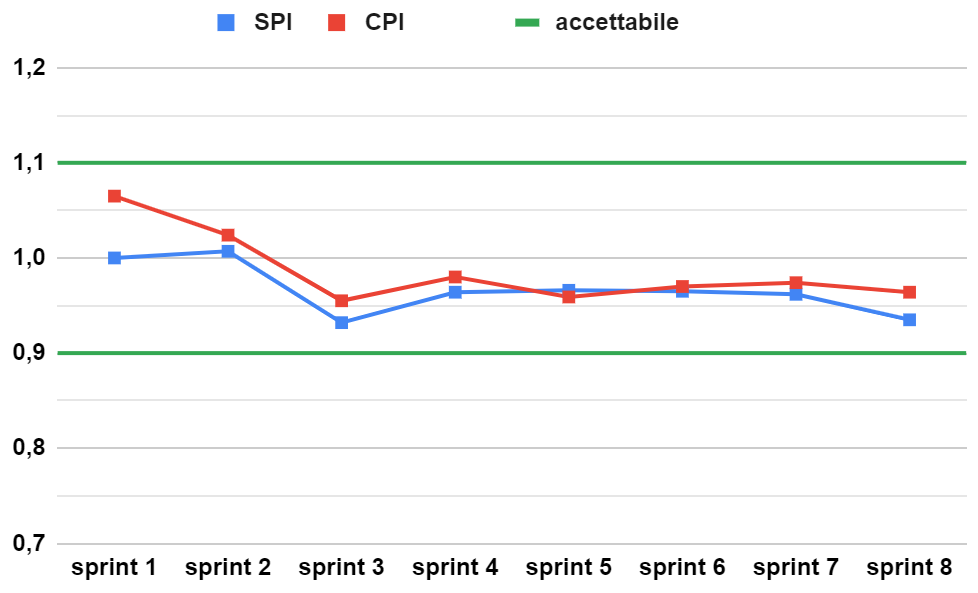
\includegraphics[width=0.8\linewidth]{SPICPI.png}
    \caption{Progressione Schedule Performance Index e Cost Performance Index}
\end{figure}
\subsection{Analisi}
Similmente a quanto riscontrabile dall'analisi dei valori di Schedule e Cost Variance, i valori di Schedule Performance Index e Cost Performance Index sono scesi sotto l'1 con la fine dello sprint 3. I valori comunque rimangono ampiamente all'interno dei valori accettabili stabilendosi sullo 0,97 fino al settimo sprint, per poi peggiorare leggermente nel periodo successivo.

\section{Misure di mitigazione insufficienti}
\begin{figure}[H]
    \centering
    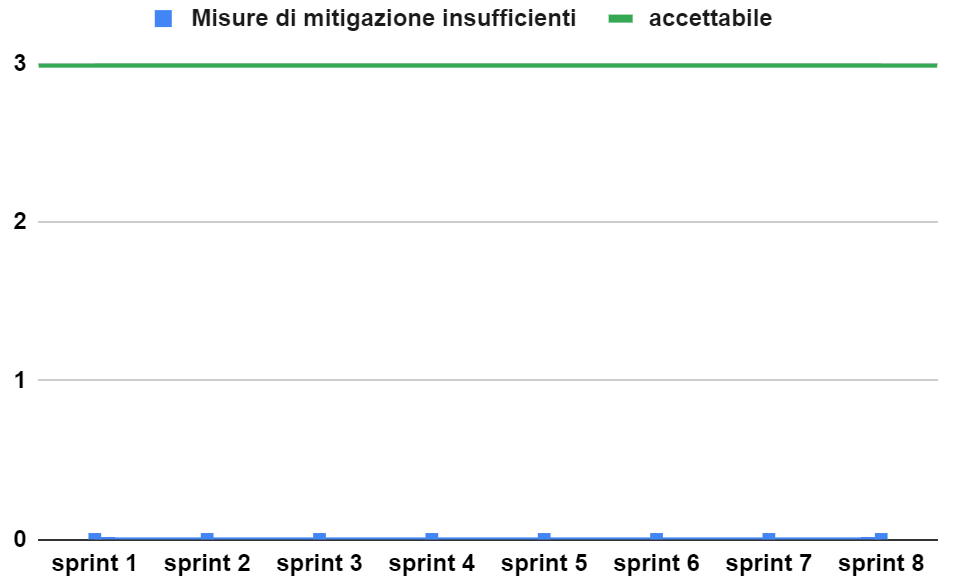
\includegraphics[width=0.8\linewidth]{Mitigazioni.png}
    \caption{Progressione occorrenza di rischi con misure mitigative insufficienti}
\end{figure}
\subsection{Analisi}
Come riscontrabile dai valori riportati dal grafico, l'ampia analisi dei rischi effettuata a inizio progetto ha portato alla definizione di misure mitigative che hanno sempre avuto efficacia.

\section{Rischi inattesi}
\begin{figure}[H]
    \centering
    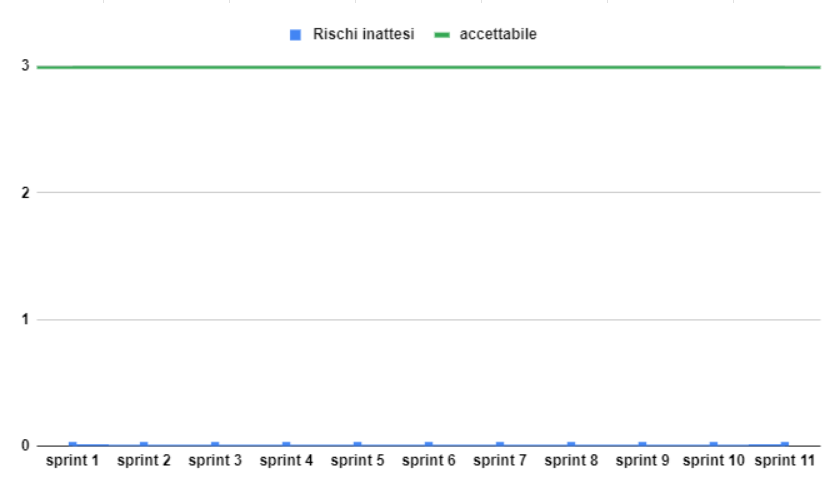
\includegraphics[width=0.8\linewidth]{Rischi.png}
    \caption{Progressione occorrenza di rischi inattesi}
\end{figure}
\subsection{Analisi}
Come osservabile dai valori riportati dal grafico, l'ampia analisi dei rischi effettuata a inizio progetto è stata soddisfacente. In particolare, nessuna problematica primaria riconoscibile come rischio è stata riscontrata fino ad ora, senza che fosse già presente nella sezione dedicata del Piano\_di\_progetto\_v2.0.

\section{Requisiti soddisfatti}
\begin{figure}[H]
    \centering
    \begin{minipage}[b]{0.32\textwidth}
        \centering
        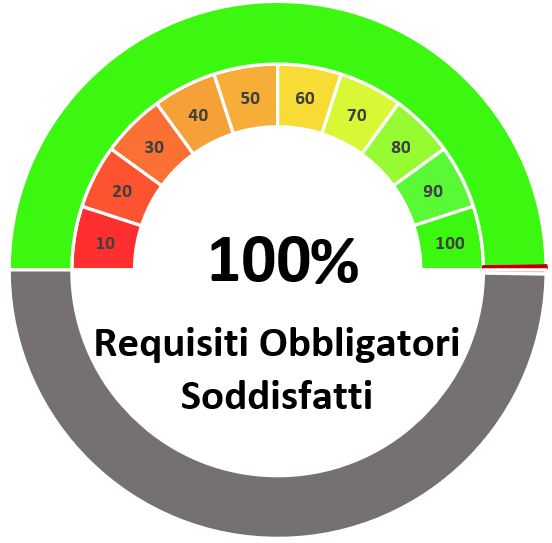
\includegraphics[width=\textwidth]{ReqObbSodd.png}
        \caption{Requisiti obbligatori soddisfatti}
        \label{reqobbsodd}
    \end{minipage}
    \hfill
    \begin{minipage}[b]{0.32\textwidth}
        \centering
        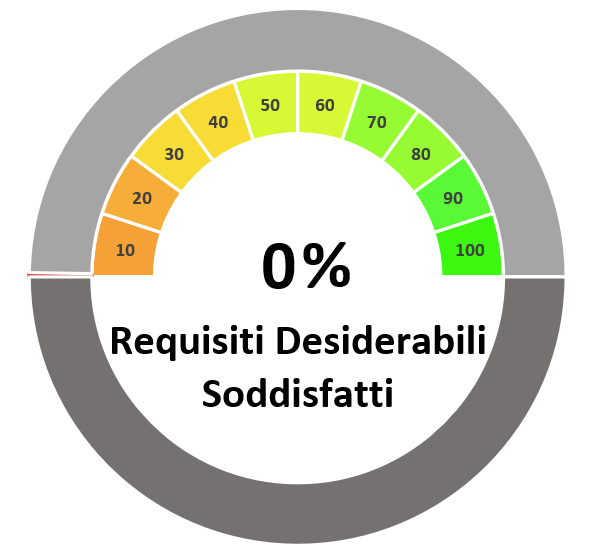
\includegraphics[width=\textwidth]{ReqDesSodd.png}
        \caption{Requisiti desiderabili soddisfatti}
        \label{reqdessodd}
    \end{minipage}
    \hfill
    \begin{minipage}[b]{0.32\textwidth}
        \centering
        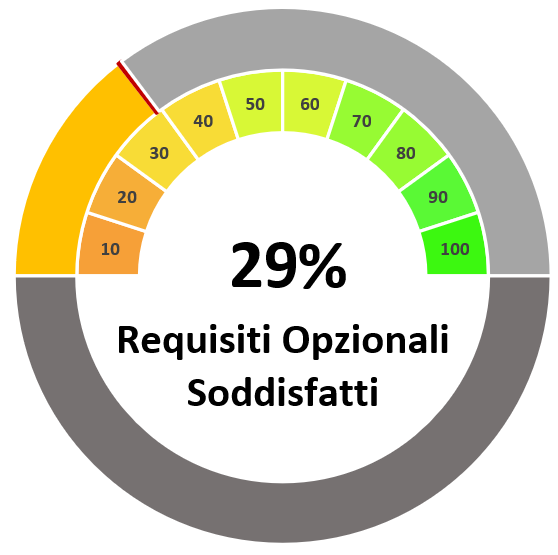
\includegraphics[width=\textwidth]{ReqOpzSodd.png}
        \caption{Requisiti opzionali soddisfatti}
        \label{reqopzsodd}
    \end{minipage}
\end{figure}
\subsection{Analisi}
Il progetto ha prodotto un Minimum Viable Product, dunque soddisfa tutti i requisiti obbligatori. Il gruppo si è inoltre dedicato a implementare anche alcuni dei requisiti desiderabili e opzionali concordati con l'azienda. La decisione di soddisfare alcuni requisiti opzionali rispetto a completare quelli desiderabili, nonostante essi siano di minor rilievo, è data dalla ridotta quantità di risorse che questi richiedevano per essere soddisfatti.
\section{Indice di Gulpease}
\begin{figure}[H]
    \centering
    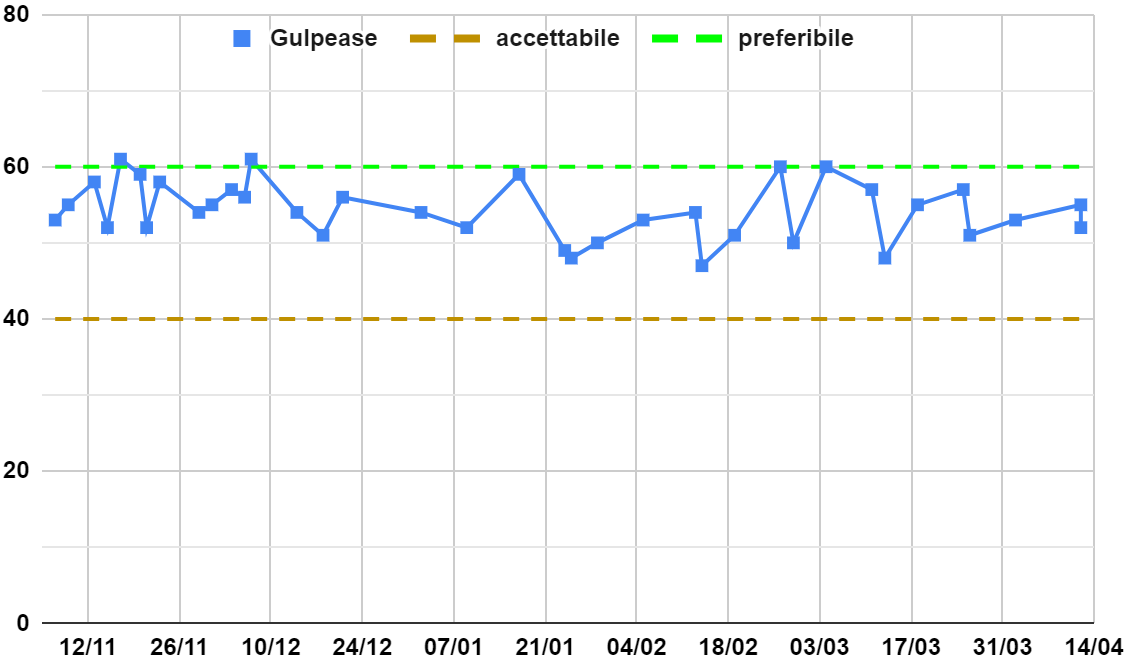
\includegraphics[width=0.8\linewidth]{GulpeaseVerbaliProgresso.png}
    \caption{Progressione indice di Gulpease dei verbali}
\end{figure}
\begin{figure}[H]
    \centering
    \begin{minipage}[b]{0.45\textwidth}
        \centering
        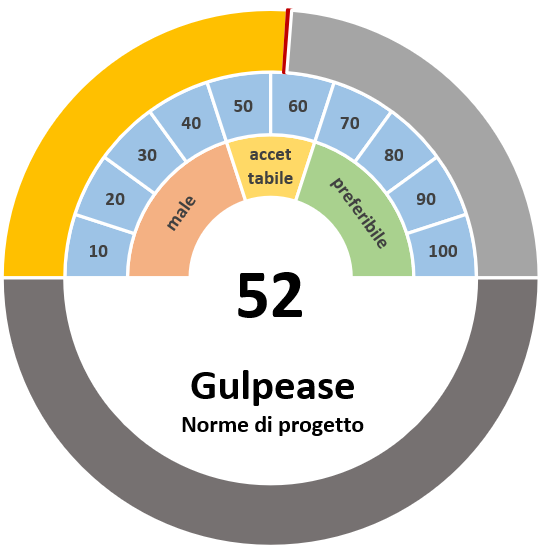
\includegraphics[width=\textwidth]{GulpeaseNdp.png}
        \caption{Gulpease di Norme\_di\_progetto\_v2.0}
    \end{minipage}
    \hfill
    \begin{minipage}[b]{0.45\textwidth}
        \centering
        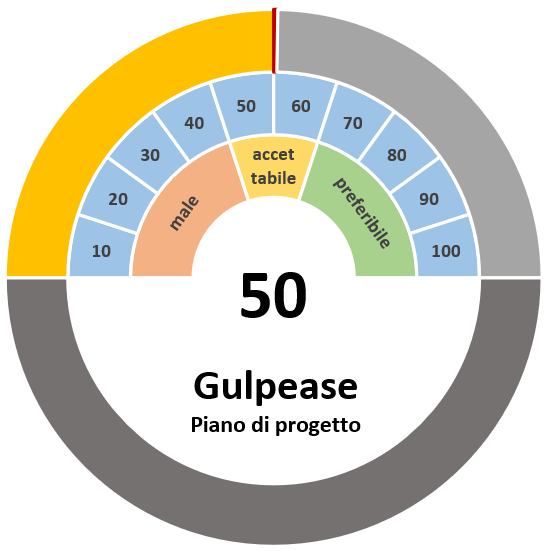
\includegraphics[width=\textwidth]{GulpeasePdp.png}
        \caption{Gulpease di Piano\_di\_progetto\_v2.0}
    \end{minipage}
\end{figure}
\begin{figure}[H]
    \centering
    \begin{minipage}[b]{0.45\textwidth}
        \centering
        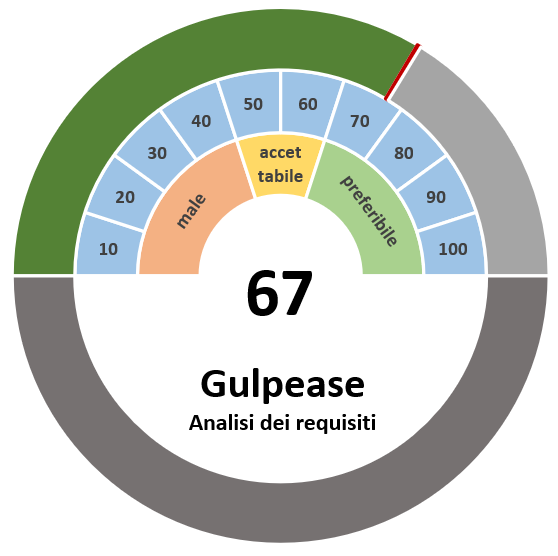
\includegraphics[width=\textwidth]{GulpeaseAdr.png}
        \caption{Gulpease di Analisi\_dei\_requisiti\_v3.0}
    \end{minipage}
    \hfill
    \begin{minipage}[b]{0.45\textwidth}
        \centering
        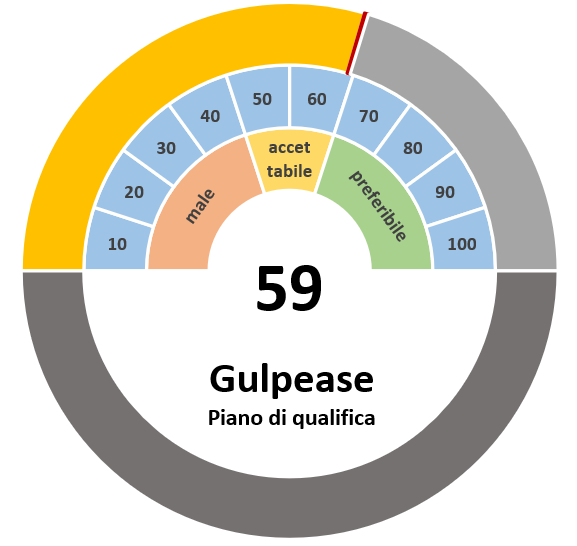
\includegraphics[width=\textwidth]{GulpeasePdq.png}
        \caption{Gulpease di Piano\_di\_qualifica\_v2.0}
    \end{minipage}
\end{figure}
\subsection{Analisi}
Analizzando i valori del cruscotto, è immediato notare che l'indice di ogni verbale è sempre stato superiore alla soglia di accettabilità. È inoltre utile notare che la maggior parte degli indici di Gulpease più bassi sono stati registrati in verbali esterni, mostrando come la natura più discorsiva di tali verbali mette a rischio maggiormente la leggibilità dei documenti.\\
L'elevata variabilità dei valori tra un documento e l'altro certifica la difficoltà nel migliorare tale metrica di qualità. Per questo motivo, è importante in futuro continuare a prestare attenzione alla struttura dei periodi delle frasi, in quanto un calo di attenzione porterebbe l'indice di un documento a non rispettare il valore di accettabilità.

\section{Code coverage}
\begin{figure}[H]
    \centering
    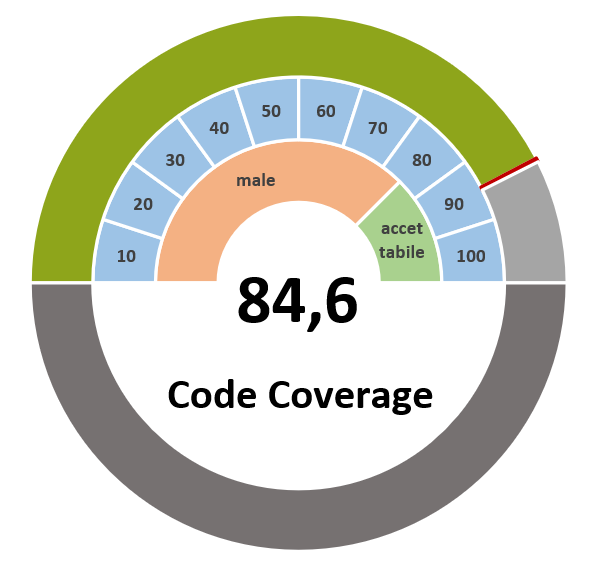
\includegraphics[width=0.45\linewidth]{codecoverage.png}
    \caption{Code coverage}
\end{figure}
\subsection{Analisi}
Il gruppo ha codificato i test di unità e di integrazione per tutte le classi del back-end e per buona parte dei componenti del front-end. I test realizzati sono stati tutti superati dall'applicazione e attraverso gli strumenti di code coverage integrati nell'ambiente di test è stato possibile raggiungere una percentuale del 84.6\%, che rispetta i valori minimi autoimposti. 